\begin{block}{one size does not fit all!}
    \begin{itemize}
        \item Tailoring guidance to specific building characteristics can improve outcomes
        \item Elevating to ``\acrshort{bfe} plus a foot'' is not always optimal \cite{xian_elevation:2017,zarekarizi_suboptimal:2020}
        \item Both over- and under-building can be costly \cite{ansar_bigisfragile:2017,DossGollin:2019}
    \end{itemize}
    \begin{framed}
        \begin{figure}
            \centering
            \begin{subfigure}{0.48\textwidth}
                \subcaption{\SI{2.5}{ft} below BFE}
                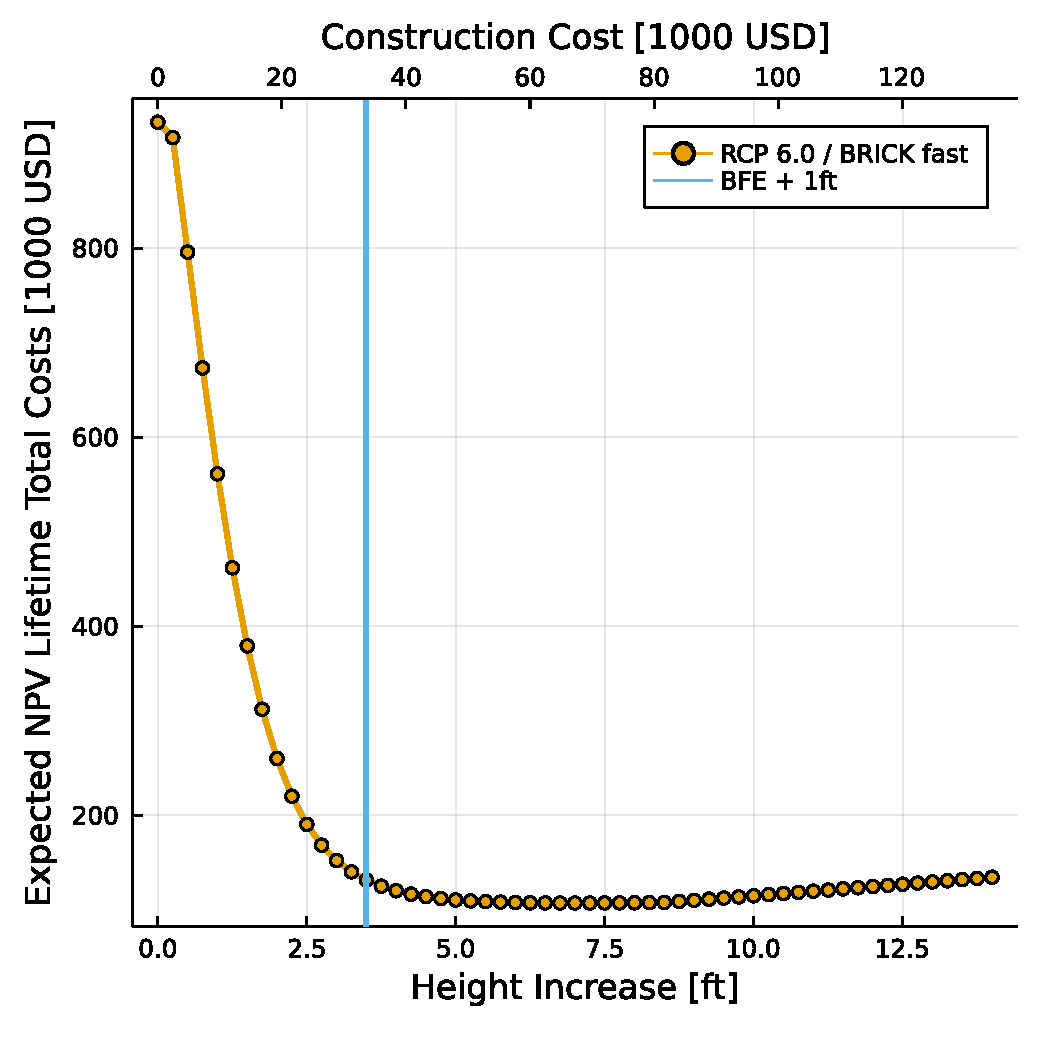
\includegraphics[width=\textwidth]{5.5.pdf}
            \end{subfigure}
            \hfill
            \begin{subfigure}{0.48\textwidth}
                \subcaption{\SI{0.5}{ft} below BFE}
                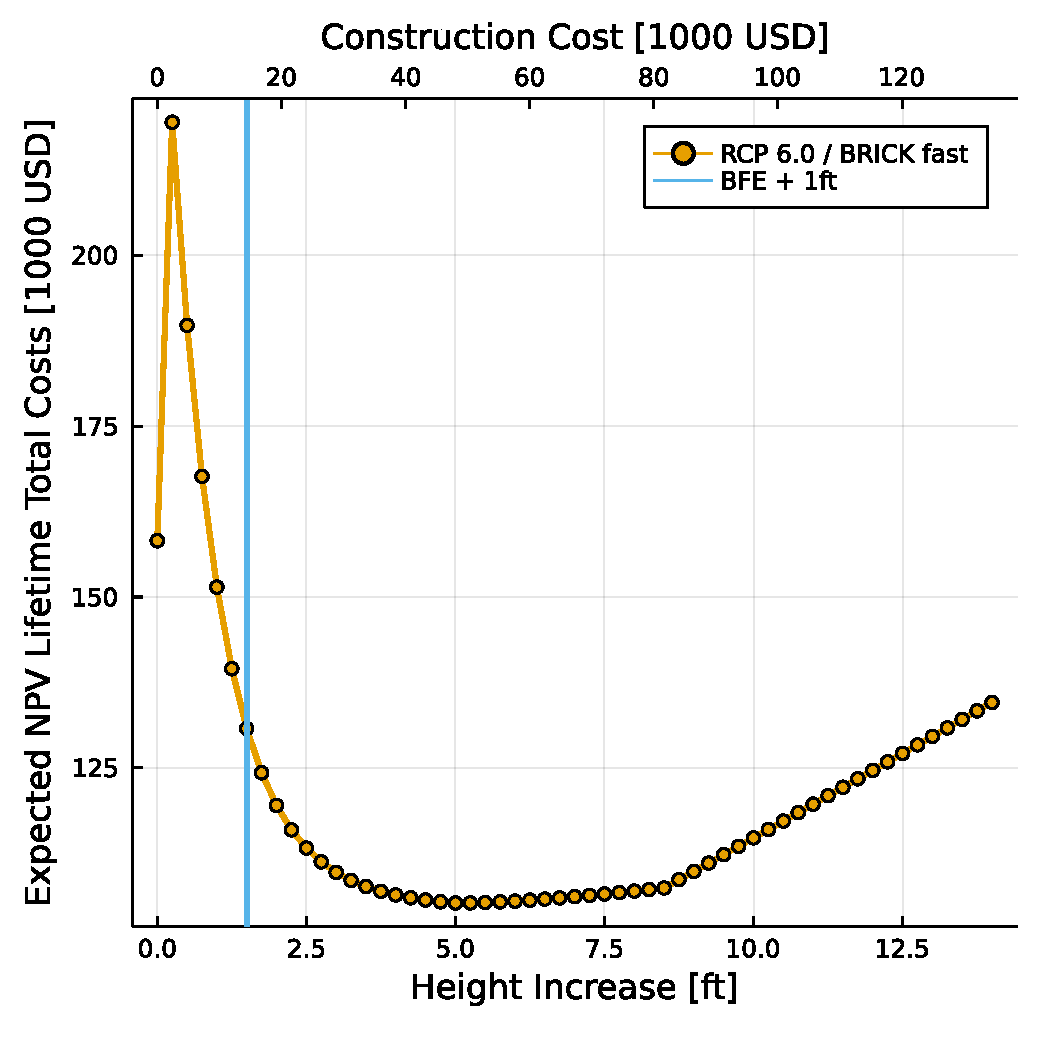
\includegraphics[width=\textwidth]{7.5.pdf}
            \end{subfigure}
            \caption{
                Tradeoffs between construction cost and expected NPV lifetime costs for houses initially situated (a) \SI{2.5}{ft} and (b) \SI{0.5}{ft} below the \gls{bfe} (under \gls{rcp} 6.0 with fast BRICK \cite{wong_brick0.2:2017} dynamics).
                Note unequal $y$-axis scales.
            }
        \end{figure}
    \end{framed}
\end{block}